\subsectiontinyvert{Architecture} \label{sec:architecture}

\begin{figure*}[thb]
\centering
% \setlength{\abovecaptionskip}{0pt plus 3pt minus 2pt}
% \setlength{\belowcaptionskip}{-35pt plus 3pt minus 2pt}
% \caption*{}
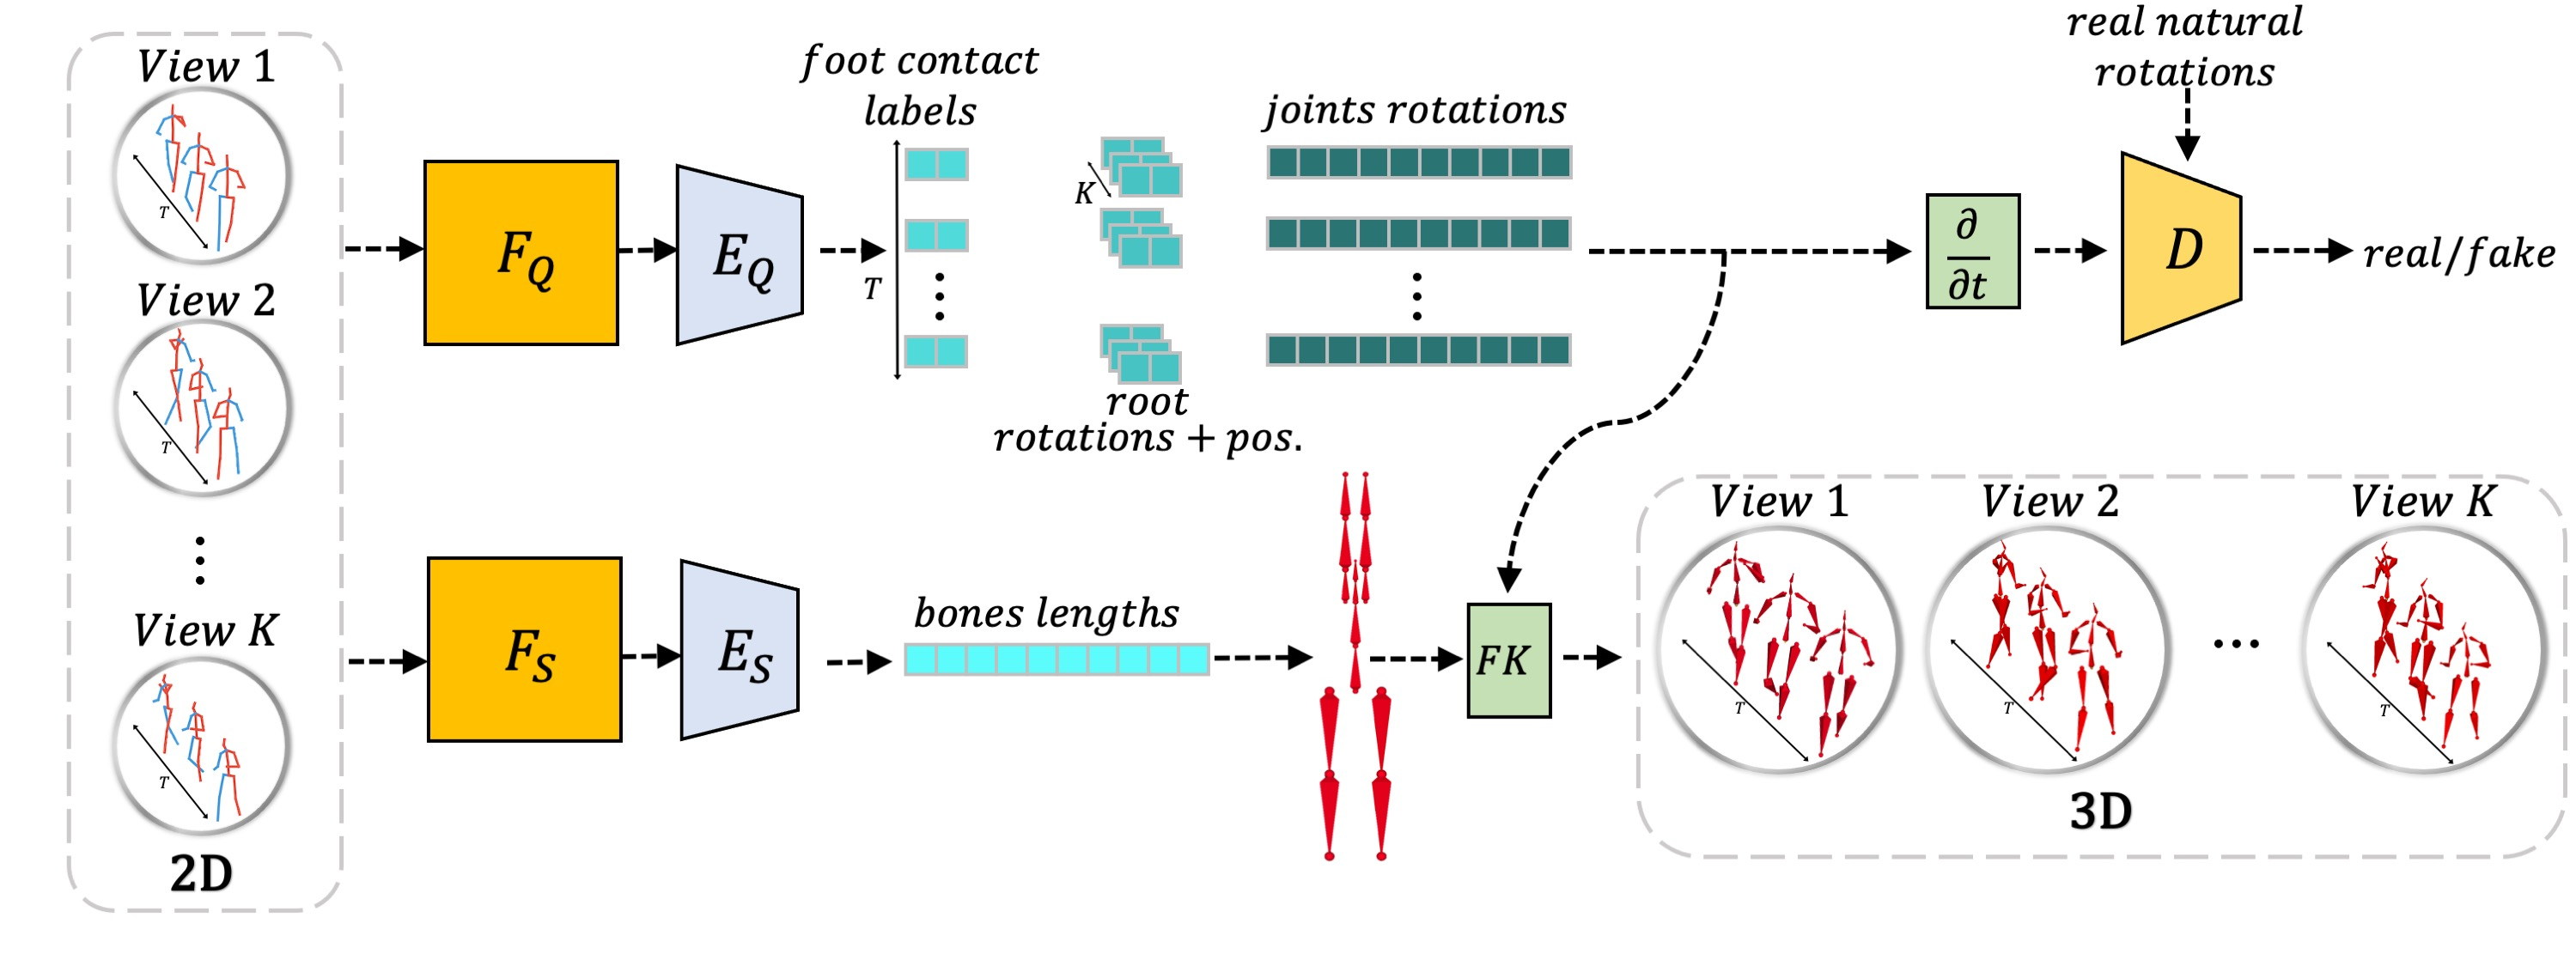
\includegraphics[width=0.9\textwidth]{./images/High_Level_Architecture.jpg}
\setlength{\abovecaptionskip}{0pt plus 3pt minus 2pt}
\setlength{\belowcaptionskip}{-15pt plus 3pt minus 2pt}
\caption{
%FLEX takes multi-view temporal sequences of 2D poses accompanied by a confidence value per joint. 
%
%Using two encoders, $E_Q$ and $E_S$, it extracts per-frame 3D joint rotations and foot contact labels, per-view and per-frame 3D root transformations, and a 3D static skeleton. 
%
%Employing a discriminator, $D$, it brings the temporal differences of rotation angles near the manifold of true rotations.
%
%Applying a forward kinematic layer, $FK$, it extracts 3D joint positions from rotations and static features, which in turn are compared to ground-truth.
%
FLEX takes multi-view temporal sequences of 2D poses and their confidence values. 
%
It uses two encoders, $E_Q$ and $E_S$, to extracts per-frame 3D rotations and foot contact labels, per-view and per-frame 3D root transformations, and one static skeleton. 
%
%
A discriminator $D$ monitors the temporal differences of rotation angles,
%
and a forward kinematic layer, $FK$, 
%extracts 3D joint locations from rotations and bone lengths,
combines encoders' outputs into 3D joint locations.
%, which in turn are compared to ground-truth.
%
\sr{These outputs depict \emph{one} human, transformed into the axis systems of $K$ cameras, to be compared with $K$ sets of  ground-truth values.}
% are identical except for their root transformation. 
% We compute $K$ outputs (rather than one) for the purpose of loss computation vs. $K$ ground-truth sets of values. 
}

\label{fig:architecture_concept}
\end{figure*}

We start with a high-level description of the architecture (see \Cref{fig:architecture_concept}). 
% Below, we point out where it diverges from MotioNet.  
%
The inputs are $K$ synchronized video streams of $T$ frames each. For each video stream, we obtain 2D joints, which are either the ground-truth of a dataset or the output of a 2D pose estimation algorithm. Our network is agnostic to the way those 2D joints were obtained. In addition, 
each estimated joint is associated with a confidence value.
The confidence value plays an important role in balancing between visible and occluded joints.

Our model takes input from all views, aggregates it, and streams it into two independent fusion layers $F_S$ and $F_Q$, followed by encoders $E_S$ and $E_Q$, respectively. The two fusion layers differ in some architectural details, but share the same concept. Both aggregate data of all views and frames and fuse it to exploit characteristics that recur in views and/or frames. Each fusion layer outputs view-agnostic features that represent the target human. 

The fusion layers consist of two innovative elements, a multi-view convolutional layer and a \emph{cross-view attention} mechanism, which encodes information from all views. Our use of attention is unique, as typically attention in other works is applied mostly over pixels~\cite{khan2021transformers} and sometimes over time~\cite{llopart2020liftformer,lin2020endtoend,liu2020attention}. 
Attention over views is a novel approach, which we find only in concurrent works for other tasks, assessing human shape \cite{zins2021datadriven} and rigid objects~\cite{wang2021multi}. \sr{The fusion  layers are described in detail in the supplementary material.}

The encoder $E_S$ predicts the length of each bone. % in the body. 
As the same human is analyzed along  all frames and views, the output is a single set of bone lengths. 

The encoder $E_Q$ predicts joint rotations, global root positions, and foot contact labels. 
Since 3D joint rotations and foot contact labels are identical to all views, $E_Q$ predicts a single set of rotations and contact labels per frame, shared by all views.
% Since 3D joint rotations are identical to all views, $E_Q$ predicts a set of rotations per frame, but not per view. 
% Similarly, foot contact label is identical per view, hence we predict a set of labels per frame but not per view.
One exception is the root (pelvis) joint, whose rotation angle and position depend on the camera view and not on the human itself. Thus, for the root joint we predict the rotation angle and position for each frame and view. Root rotation and position are relative to the camera; hence visualizing the reconstructed object depicts the filmed person from the camera view, as expected.
Notice that root rotation and position carry the knowledge of the relative transformation between the cameras.
This insight suggests that our algorithm has the potential to output additional valuable information, \eg, cameras relative location to each other (left to future work).

At train time, the output of both encoders is combined in $K$ identical forward kinematic ($FK$) layers. 
Each $FK$ layer computes the estimated 3D joint positions related to one view, which in turn are 
 compared to the ground-truth for loss computation. 
In addition, temporal differences of the rotations extracted out of $E_Q$, are fed to a discriminator $D$~\cite{Kanazawa:2018}, so they get near the manifold of true rotations in an adversarial way. 
%\sr{The outputs of all $FK$ layers are equivalent to each other and depict the same motion, relative to the axis systems of $K$ cameras. We compute $K$ outputs solely for the purpose of loss computation vs. GT values of the cameras in the dataset.}
%At inference time, bone lengths, joint rotations and global root positions constitute a complete description of a motion.

% Additionally to introducing fusion layers, FLEX changes the building blocks of MotioNet as follows. Our input is an aggregation of all views, whereas MotioNet takes each view separately. The encoders, $E_S$ and $E_Q$, now take their input from the fusion layers, requiring a change in their architecture. Lastly, the output is changed to contain a root transformation per view in addition to Motionet's outputs.
%The output, however, remains lean (no extra view information), except for an addition of root transformation per view.

%We now proceed into a more formal description. Throughout the description, we make an effort to match the notation of the baseline~\cite{shi2020motionet}, up to points where the models depart.
%
% Let 
\sr{Formally,} let $\bL$ denote the number of bones, $\bT$ the temporal length of the sequence, $\bJ$ the number of joints, $\bQ$ the size of the rotations representation vector, and $\bK$ the number of cameras.
%
Let $\bP_{s,q,r}\in
\bbr
^{T\times 3J\times K}$ 
denote $K$ temporal sequences of 3D joint positions generated by a skeleton $\bss\in\bbr^L$ with joint rotations $\bq\in\bbr^{T\times Q\times(J-1)}$, and global root position and rotation $\br\in\bbr^{T\times (3+Q)\times K}$. Note that $q$ is related to all joints except for the root joint. The rotation of the root joint, as well as its position, are related to $r$. 

Our approach expects an input $\bV_{s,q,r}\in\bbr^{T\times 3J\times K}$ denoting $K$ temporal sequences of 2D joints and a confidence value per joint, 
related to a skeleton $s$, joint rotations $q$, and global root position and rotation $r$. 
Each input $V$ is fed into our deep neural network, which in turn predicts $\tilde{\bq}\in\mathbb{R}^{T\times Q\times(J-1)}$, that captures the dynamic, rotational information of the motion, $\tilde{\bss}\in\mathbb{R}^L$, that describes a single, consistent, skeleton, $\tilde{\br}\in\mathbb{R}^{T\times (3+Q)\times K}$ that estimates the global position and rotation of the root along time and along views, and $\tilde{\bff}\in\{0,1\}^{T\times 2}$ that predicts whether each of the two feet touches the ground in each frame:
%We have that 

\setlength{\abovedisplayskip}{-5pt plus 2pt minus 2pt}
\setlength{\belowdisplayskip}{5pt plus 2pt minus 2pt}

\begin{align}
\tilde{\bss} = E_S(F_S(\bV_{s,q,r})) ,  ~~~~~~~~~~
\tilde{\bq},\tilde{\br},\tilde{\bff} = E_Q(F_Q(\bV_{s,q,r})).
\end{align}
These attributes can be then combined via forward kinematics to estimate $K$ global 3D pose sequences, $\tilde{\bP}_{\tilde{s},\tilde{q},\tilde{r}}\in\mathbb{R}^{T\times 3J\times K}$, specified by joint positions:

\setlength{\abovedisplayskip}{-5pt plus 2pt minus 2pt}
\setlength{\belowdisplayskip}{5pt plus 2pt minus 2pt}

\begin{align}
\tilde{\bP}_{\tilde{s},\tilde{q},\tilde{r}}=FK(\tilde{\bss}, \tilde{\bq}, \tilde{\br}).
\end{align}

%FLEX is not limited to a specific rotation representation. Rotations can be expressed by Euler angles, exponential maps~\cite{grassia1998practical}, unit quaternions, 6D representation~\cite{Zhou_2019_CVPR}, rotation matrices, and more. Following the considerations raised by Shi \etal~\shortcite{shi2020motionet}, we choose to use unit quaternions.

%%%%%%%%%%

